
%(BEGIN_QUESTION)
% Copyright 2006, Tony R. Kuphaldt, released under the Creative Commons Attribution License (v 1.0)
% This means you may do almost anything with this work of mine, so long as you give me proper credit

Determine the correct potentiometer millivoltage setting to generate the following temperature indications on the following instruments:

$$\includegraphics[width=15.5cm]{i00388x01.eps}$$

\begin{itemize}
\item{} 0$^{o}$ F ; Potentiometer setting = ??? 
\item{} 300$^{o}$ F ; Potentiometer setting = ??? 
\item{} 600$^{o}$ F ; Potentiometer setting = ??? 
\end{itemize}

\vskip 10pt

$$\includegraphics[width=15.5cm]{i00388x02.eps}$$

\begin{itemize}
\item{} 400$^{o}$ F ; Potentiometer setting = ??? 
\item{} 600$^{o}$ F ; Potentiometer setting = ??? 
\item{} 800$^{o}$ F ; Potentiometer setting = ??? 
\end{itemize}

\vskip 10pt

$$\includegraphics[width=15.5cm]{i00388x03.eps}$$

\begin{itemize}
\item{} 250$^{o}$ F ; Potentiometer setting = ??? 
\item{} 500$^{o}$ F ; Potentiometer setting = ??? 
\item{} 750$^{o}$ F ; Potentiometer setting = ??? 
\end{itemize}

\vskip 20pt \vbox{\hrule \hbox{\strut \vrule{} {\bf Suggestions for Socratic discussion} \vrule} \hrule}

\begin{itemize}
\item{} In each of these example circuits, only one of the ambient temperatures given is relevant.  Identify which one that is, and explain why the other one doesn't matter.
\item{} What would have to be different in each circuit for the irrelevant temperature to matter?
\item{} Explain what you would have to alter in each circuit in order to disable the temperature instrument's cold junction compensation (CJC).
\end{itemize}

\underbar{file i00388}
%(END_QUESTION)





%(BEGIN_ANSWER)

\noindent
{\bf Partial answer:}

\begin{itemize}
\item{} {\bf Type K}
%\item{} 0$^{o}$ F ; Potentiometer setting = -1.670 mV 
\item{} 300$^{o}$ F ; Potentiometer setting = 5.116 mV 
%\item{} 600$^{o}$ F ; Potentiometer setting = 11.877 mV 
\medskip

\vskip 10pt

\begin{itemize}
\item{} {\bf Type J}
\item{} 400$^{o}$ F ; Potentiometer setting = 10.006 mV 
%\item{} 600$^{o}$ F ; Potentiometer setting = 16.169 mV 
%\item{} 800$^{o}$ F ; Potentiometer setting = 22.301 mV 
\medskip

\vskip 10pt

\begin{itemize}
\item{} {\bf Type J}
%\item{} 250$^{o}$ F ; Potentiometer setting = 5.914 mV
%\item{} 500$^{o}$ F ; Potentiometer setting = 13.603 mV 
\item{} 750$^{o}$ F ; Potentiometer setting = 21.280 mV
\end{itemize}

%(END_ANSWER)





%(BEGIN_NOTES)

In the first example, the ambient temperature of interest is 76 $^{o}$F, because that is where the reference compensation thermistor is located.  For a type K thermocouple at this temperature, the reference junction voltage would be 0.978 millivolts.  Therefore, this is the amount of voltage we must subtract from the desired temperature's voltage before setting the precision potentiometer:

\begin{itemize}
\item{} {\bf Type K}
\item{} 0$^{o}$ F ; Potentiometer setting = $-$0.692 mV $-$ 0.978 mV = {\bf $-$1.670 mV}
\item{} 300$^{o}$ F ; Potentiometer setting = 6.094 mV $-$ 0.978 mV = {\bf 5.116 mV} 
\item{} 600$^{o}$ F ; Potentiometer setting = 12.855 mV $-$ 0.978 mV = {\bf 11.877 mV}
\end{itemize}

\vskip 10pt

In the second example, the ambient temperature of interest is 68 $^{o}$F, because that is where the reference compensation thermistor is located.  For a type J thermocouple at this temperature, the reference junction voltage would be 1.019 millivolts.  Therefore, this is the amount of voltage we must subtract from the desired temperature's voltage before setting the precision potentiometer:

\begin{itemize}
\item{} {\bf Type J}
\item{} 400$^{o}$ F ; Potentiometer setting = 11.025 mV $-$ 1.019 mV = {\bf 10.006 mV}
\item{} 600$^{o}$ F ; Potentiometer setting = 17.188 mV $-$ 1.019 mV = {\bf 16.169 mV} 
\item{} 800$^{o}$ F ; Potentiometer setting = 23.320 mV $-$ 1.019 mV = {\bf 22.301 mV} 
\end{itemize}

\vskip 10pt

In the third example, the ambient temperature of interest is 50 $^{o}$F, because that is where the additive thermocouple junction is located.  There is a (subtractive) reference junction located at the receiving instrument, but its voltage is canceled by the compensating thermistor bridge and therefore is of no concern.  The presence of a real thermocouple junction at the precision potentiometer basically does the same thing that a compensating network does when there is no reference junction to compensate for: it adds an unwanted voltage to the input of the receiving instrument.  For a type J thermocouple at 50 $^{o}$F, this junction voltage is 0.507 millivolts.  Therefore, this is the amount of voltage we must subtract from the desired temperature's voltage before setting the precision potentiometer:

\begin{itemize}
\item{} {\bf Type J}
\item{} 250$^{o}$ F ; Potentiometer setting = 6.421 mV $-$ 0.507 mV = {\bf 5.914 mV} 
\item{} 500$^{o}$ F ; Potentiometer setting = 14.110 mV $-$ 0.507 mV = {\bf 13.603 mV} 
\item{} 750$^{o}$ F ; Potentiometer setting = 21.787 mV $-$ 0.507 mV = {\bf 21.280 mV}
\end{itemize}
















\vfil \eject

\noindent
{\bf Summary Quiz:}

Referencing a table of millivoltage values for type N thermocouples (ITS-90), determine the amount of millivoltage a technician must apply to the input terminals of a type N thermocouple transmitter to make that transmitter ``think'' it is connected to a thermocouple at a process temperature of 320 degrees Fahrenheit.  Assume the transmitter itself is situated in a room at an ambient temperature of 70 degrees Fahrenheit.

%INDEX% Measurement, temperature: thermocouple millivoltage calibration

%(END_NOTES)


